\documentclass[border=10pt,tikz]{standalone}
\usepackage[document]{ragged2e}
\usetikzlibrary{angles,quotes}
\usetikzlibrary[calc]
\begin{document}
  
\hyphenchar\font=-1

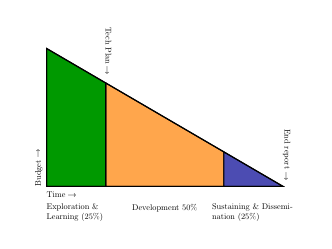
\begin{tikzpicture}[
  my angle/.style={
    every pic quotes/.append style={text=cyan},
    draw=cyan,
    angle radius=1cm,
  }]
  \coordinate (C) at (-1.5,-1);
  \coordinate (A) at (1.5,-1); 
%  \coordinate [label=below left:$A$] (A) at (1.5,-1);  
  \coordinate (B) at (-1.5,0.75); 
%  \coordinate [label=above:$B$] (B) at (-1.5,0.75);   
  \coordinate (AB1) at ($(A)!.25!(B)$);
  \coordinate (AB2) at ($(A)!.75!(B)$);  
  \coordinate (AC1) at ($(A)!.25!(C)$);
  \coordinate (AC2) at ($(A)!.75!(C)$);  
  \draw [fill=orange!70] (AB1) to (AB2) to (AC2) to (AC1) to cycle;
  \draw [fill=green!60!black] (C) to (B) to (AB2) to (AC2) to node[below,yshift=-1mm] {\scalebox{0.3}{\parbox[t][0pt]{2.5cm}{Exploration \& Learning (25\%)}}} cycle;  
  \draw [fill=blue!40!gray] (AC1) to (AB1) to (A) to node[below,yshift=-1mm] {\scalebox{0.3}{\parbox[t][0pt]{3.5cm}{Sustaining \& Dissemination (25\%)}}} cycle;   
  \draw (C) -- node[left] {} (B) -- node[above] {} (A) -- node[below,yshift=-1mm] {\scalebox{0.3}{Development 50\%}} (C);
  \node [below of=C, node distance=1mm,xshift=0,anchor=west, rectangle,inner sep=0,outer sep=0] {\scalebox{0.3}{Time \textrightarrow}};
  \node [left of=C, node distance=1mm,xshift=0,anchor=west, rectangle,inner sep=0,outer sep=0,rotate=90] {\scalebox{0.3}{Budget \textrightarrow}};
  \node [left of=AB2, node distance=1mm,xshift=1mm,yshift=4mm,anchor=south, rectangle,inner sep=0,outer sep=0,rotate=-90] {\scalebox{0.3}{Tech Plan \textrightarrow}};  
  \node [above of=A, node distance=1mm,xshift=0mm,yshift=3mm,anchor=south, rectangle,inner sep=0,outer sep=0,rotate=-90] {\scalebox{0.3}{End report \textrightarrow}};  
  %\draw (AB1) -- (AC1);
  %\draw (A) +(-.25,0) |- +(0,.25);
  %\pic [my angle, "$\alpha$"] {angle=A--C--B};
  %\pic [my angle, "$\beta$"] {angle=C--B--A};
\end{tikzpicture}
\end{document}\end{document}